\documentclass[12pt,a4paper]{report}

\usepackage[T1]{fontenc}
\usepackage[a4paper,left=1.5in,right=1.25in,top=1.25in,bottom=1.25in,headheight=15pt]{geometry}
\usepackage{mathptmx}
\usepackage{array}
\usepackage{tabularx}
\usepackage{booktabs}
\usepackage[table]{xcolor}
\usepackage{graphicx}
\usepackage{float}
\usepackage{enumitem}
\usepackage{setspace}
\usepackage{fancyhdr}
\usepackage{titlesec}
\usepackage{caption}
\usepackage{hyperref}
\usepackage{xurl}
\usepackage{tikz}
\usetikzlibrary{arrows.meta,positioning,fit}

\graphicspath{{./images/}{./}}
\urlstyle{same}

\hypersetup{
    colorlinks=true,
    linkcolor=black,
    citecolor=black,
    urlcolor=blue,
    breaklinks=true,
    pdftitle={MarketGyan: NEPSE and Financial News Analysis},
    pdfauthor={Bikash Kumar Sah}
}

\onehalfspacing
\setlength{\parindent}{0pt}
\setlength{\parskip}{8pt}
\setlength{\emergencystretch}{2em}

\pagestyle{fancy}
\fancyhf{}
\fancyfoot[C]{\thepage}
\renewcommand{\headrulewidth}{0pt}
\renewcommand{\bibname}{References}
\newcolumntype{Y}{>{\raggedright\arraybackslash}X}
\newcolumntype{L}[1]{>{\raggedright\arraybackslash}p{#1}}

\titleformat{\chapter}[display]
{\normalfont\bfseries\Large\centering}
{\chaptername\ \thechapter}{10pt}{\Large}
% Normalize the vertical space above/below every chapter title so all chapters
% (and the unnumbered front-matter chapters) start at the same height.
\titlespacing*{\chapter}{0pt}{10pt}{20pt}
\titleformat{\section}
{\normalfont\bfseries\large}{\thesection}{1em}{}
\titleformat{\subsection}
{\normalfont\bfseries\normalsize}{\thesubsection}{1em}{}

\newcommand{\studentname}{Bikash Kumar Sah}
\newcommand{\rollnumber}{16}
\newcommand{\programname}{B.Tech in Artificial Intelligence}
\newcommand{\semesterinfo}{IV Year, I Semester}
\newcommand{\submissiondate}{July 3, 2026}
\newcommand{\projecttitle}{MarketGyan: NEPSE and Financial News Analysis}
\newcommand{\projectsubtitle}{An Extension of Khabar AI}
\newcommand{\supervisorone}{Mr. Sundeep Gupta}
\newcommand{\supervisortwo}{Ms. Sristi Khatiwada}

\newcommand{\insertkulogo}{%
    \IfFileExists{images/ku.png}{\includegraphics[scale=0.12]{images/ku.png}}{%
    \IfFileExists{ku.png}{\includegraphics[scale=0.12]{ku.png}}{%
    \IfFileExists{ku_logo.png}{\includegraphics[scale=0.12]{ku_logo.png}}{%
    \IfFileExists{images/ku_logo.png}{\includegraphics[scale=0.12]{images/ku_logo.png}}{%
        \vspace{1.0cm}%
    }}}}%
}

\begin{document}

\begin{titlepage}
    \thispagestyle{empty}
    \begin{center}
        \huge \textbf{Kathmandu University}\\[6pt]
        \Large \textbf{School of Engineering}\\[6pt]
        \Large \textbf{Department of Artificial Intelligence}\\
        \large \textbf{Dhulikhel, Kavre}\\[10pt]

        \insertkulogo\par\vspace{8pt}

        \large \textbf{Semester Project Final Report}\\[2pt]
        \large In partial fulfillment of the requirements for\\
        \large \semesterinfo\ of \programname\\[12pt]

        \rule{\textwidth}{0.6pt}\\[6pt]
        \begin{minipage}{0.93\textwidth}
            \centering
            \fontsize{14}{16}\selectfont\textbf{\projecttitle}\\[2pt]
            \fontsize{14}{16}\selectfont\textbf{\projectsubtitle}
        \end{minipage}\\[6pt]
        \rule{\textwidth}{0.6pt}\\[16pt]
        \vspace{0.4cm}

        \begin{tabular}{rl}
            \textbf{Submitted by:} & \studentname \\
            \textbf{Roll Number:} & \rollnumber \\
            \textbf{Submission Date:} & \submissiondate \\
        \end{tabular}

        \vspace{0.8cm}

        \textbf{Submitted to}\\
        Head of Department\\
        Department of Artificial Intelligence
    \end{center}
\end{titlepage}

\pagenumbering{roman}

\chapter*{Abstract}
\addcontentsline{toc}{chapter}{Abstract}
MarketGyan is a Nepal-focused financial natural language processing project that extends the Khabar AI news platform into a market-analysis assistant for the Nepal Stock Exchange (NEPSE). The project combines public market snapshots, local financial news, regulatory documents, a bilingual human-adjudicated benchmark, supervised baselines, a fine-tuned Qwen3.5-9B LoRA adapter, and a retrieval-augmented generation runtime. Its main research artifact is NEPSE-Impact-500: a 500-row English and Nepali benchmark for identifying whether Nepal-focused news is relevant to NEPSE, classifying event type and potential market direction, mapping entities to sectors and symbols, and grounding each label in numbered evidence sentences.

The project first trained a multilingual XLM-R baseline on the frozen benchmark. XLM-R relevance classification reached 0.813 accuracy and 0.743 macro-F1 on the 75-row test split, while relevant-record direction classification reached 0.567 accuracy and 0.568 macro-F1 on the merged three-class direction target. A small English-only FinBERT sanity baseline reached 0.889 accuracy and 0.616 macro-F1 on the English relevant subset. The final Qwen3.5-9B targeted-v2 adapter improved the structured extraction path, reaching 1.000 strict structured-output validity, 1.000 evidence grounding, 0.840 relevance accuracy, and 0.796 relevance macro-F1 on the same frozen test split. The frontend demonstrates grounded Qwen answers, evidence search, and local report generation. At the same time, neutral direction recall, sector recall, symbol recall, and evidence-recall remain weak. The final contribution is therefore best understood as a demo-ready research prototype with a reproducible benchmark and clear technical limitations, not as a production financial advisory system.

\vspace{6pt}
\noindent\textbf{Keywords:} NEPSE, Financial NLP, Low-Resource Languages, Nepali, Retrieval-Augmented Generation, LoRA Fine-Tuning, XLM-R, Qwen, Evidence Grounding, Benchmark Dataset.

\chapter*{Acknowledgement}
\addcontentsline{toc}{chapter}{Acknowledgement}
I would like to express sincere gratitude to the Department of Artificial Intelligence, Kathmandu University, for providing the academic structure for this semester project. I am especially thankful to my supervisors, \supervisorone{} and \supervisortwo{}, for their guidance, review, and support throughout the development of MarketGyan. Their feedback helped narrow the project from a broad financial assistant into a measurable Nepal-specific financial NLP and retrieval system.

I am also thankful to the faculty members and project reviewers whose comments improved the benchmark, evaluation plan, and final system demonstration. Public market and regulatory sources, including NEPSE, ShareSansar, Nepal Rastra Bank, and SEBON, made the research prototype possible through publicly available data. Finally, I would like to thank everyone who supported the annotation, testing, and review process during the final project phase.

\vspace{1.4cm}
\begin{tabularx}{\textwidth}{@{}X X@{}}
\textbf{Supervisor Signature} & \textbf{Supervisor Signature} \\[1.2cm]
\hrulefill & \hrulefill \\
\supervisorone{} & \supervisortwo{} \\
Date: \hrulefill & Date: \hrulefill \\
\end{tabularx}

\tableofcontents
\clearpage

\listoffigures
\addcontentsline{toc}{chapter}{List of Figures}
\clearpage

\listoftables
\addcontentsline{toc}{chapter}{List of Tables}
\clearpage

\chapter*{List of Abbreviations}
\addcontentsline{toc}{chapter}{List of Abbreviations}
\begin{tabular}{ll}
AI & Artificial Intelligence \\
API & Application Programming Interface \\
BF16 & Brain Floating Point 16-bit \\
F1 & F1-Score \\
JSON & JavaScript Object Notation \\
LLM & Large Language Model \\
LoRA & Low-Rank Adaptation \\
NEPSE & Nepal Stock Exchange \\
NLP & Natural Language Processing \\
NRB & Nepal Rastra Bank \\
P@5 & Precision at 5 \\
QLoRA & Quantized Low-Rank Adaptation \\
RAG & Retrieval-Augmented Generation \\
SEBON & Securities Board of Nepal \\
UI & User Interface \\
vLLM & Virtual Large Language Model serving engine \\
\end{tabular}
\clearpage

\pagenumbering{arabic}

\chapter{Introduction}

\section{Background}
Investors in Nepal follow daily market movement through NEPSE market summaries, broker portals, financial news websites, regulatory circulars, and social media discussions. These sources are fragmented. A user who wants to understand a single trading day must manually connect index movement, sector performance, company-specific announcements, monetary policy, regulation, and news sentiment. General news summarizers are not enough for this task because financial interpretation depends on market relevance, listed-company identification, event type, potential direction, and evidence quality.

MarketGyan extends the existing Khabar AI platform into this financial-analysis domain. Instead of building a separate application from the beginning, the project reuses the existing news ingestion, scheduler, backend, semantic search, and React frontend foundations. The new contribution is a finance-specific data pipeline, benchmark, model, retrieval contract, citation validation path, and local demonstration workflow.

\section{Problem Statement}
The project problem is to design and evaluate a Nepal-specific financial NLP system that can combine structured market data with local financial news and regulatory updates. The system should identify which articles are relevant to NEPSE, classify their likely market impact, retrieve supporting evidence, and generate grounded answers or daily reports without giving buy or sell advice. The work is a research prototype and demonstration system, not a production trading platform.

\section{Objectives}

\subsection{General Objective}
The general objective of this project is to design, build, and evaluate a Nepal-specific financial NLP research prototype that combines structured NEPSE market data with local financial news and regulatory updates to produce evidence-grounded market analysis without giving buy or sell advice.

\subsection{Specific Objectives}
The specific objectives were:
\begin{enumerate}[leftmargin=1.7em]
    \item extend Khabar AI to collect and manage NEPSE-related market data, financial news, and selected regulatory sources;
    \item create a bilingual, human-adjudicated benchmark for NEPSE news relevance and potential impact;
    \item fine-tune and evaluate a 7B--10B class instruction model for structured financial impact extraction; and
    \item build a RAG runtime that answers user queries and generates reports with evidence citations.
\end{enumerate}

\section{Scope}
The system uses public market data, public news, and public regulatory sources. It covers daily NEPSE market snapshots, sector-level market context, finance-focused news articles, selected NRB and SEBON regulatory material when machine-readable text is available, and archived MarketGyan reports. The model scope is limited to news relevance, event type, potential impact direction, affected sectors or symbols, and evidence sentence selection. The application scope includes evidence search, grounded question answering, and local report generation inside the existing Khabar AI dashboard.

The project deliberately excludes trading execution, brokerage integration, portfolio optimization, personal risk profiling, price forecasting, and direct buy or sell recommendations. It also excludes unreadable legacy-font PDFs and OCR-heavy regulatory extraction from the final deliverable because those files require a separate document-processing track. MarketGyan is therefore an informational research prototype: it can explain what public evidence says about market events, but it does not claim to predict returns or provide investment advice.

The evaluation scope is also bounded. The frozen 500-row benchmark measures model behavior on curated English and Nepali article examples. These tests are sufficient for an academic prototype evaluation, but they are not equivalent to production reliability testing across all Nepal-market news sources and trading dates.

\chapter{Related Work}

\section{Nepali and Multilingual NLP}
Work on Nepali NLP remains more limited than work on high-resource languages, but recent studies provide a stronger foundation than was available even a few years ago. Timilsina et al. introduced NepBERTa, a monolingual Nepali language model trained on a large news corpus, and showed that language-specific pre-training improves multiple Nepali NLP tasks \cite{timilsina2022}. Subedi et al. evaluated large language models for Nepali named-entity recognition and part-of-speech tagging, highlighting both the promise of modern transformer models and the continuing importance of low-resource benchmarks \cite{subedi2024}. Thapa et al. expanded the Nepali model landscape by training new encoder and decoder models on a substantially larger monolingual corpus and reporting gains on both understanding and generation tasks \cite{thapa2025}. These studies suggest that Nepali text can now be processed more directly in applied systems, especially when multilingual or Nepali-adapted models are combined with careful fine-tuning and task-specific evaluation. MarketGyan follows this direction by treating Nepali and English financial articles as first-class benchmark inputs rather than translating everything into English.

\section{Financial NLP and Financial LLMs}
Financial text differs from general news because it contains domain-specific terminology, event-driven sentiment, and interpretation that depends on policy, regulation, and sector context. MarketGyan is positioned within this financial NLP line of work, but it narrows the problem to Nepal-market relevance, potential impact, and evidence-grounded structured extraction.

\subsection{FinBERT: Domain-Specific Financial Sentiment}
FinBERT established that adapting a transformer model to financial language improves financial sentiment classification compared with using a general-purpose language model directly \cite{araci2019finbert}. This is important for MarketGyan because the same word can imply different direction depending on financial context. For example, a capital raise, a regulatory notice, or a liquidity update cannot be judged only by generic positive or negative wording. The project therefore includes an English-only FinBERT sanity baseline while recognizing that it cannot cover Nepali articles or the full structured NEPSE impact schema.

\subsection{FinGPT: Data-Centric Financial LLM Adaptation}
FinGPT emphasizes that financial LLM performance depends heavily on data curation, lightweight adaptation, and task-specific instruction data \cite{yang2023fingpt}. MarketGyan adopts this data-centric view. The main contribution is not the LoRA method itself, but the curated NEPSE-Impact-500 benchmark, hard-negative relevance examples, sentence-grounded evidence labels, and Nepal-specific event ontology. This choice also explains why the final improvement path focuses on benchmark quality, retrieval metadata, and evidence selection rather than simply increasing model size.

\subsection{FinLLM Survey: Benchmarks, Hallucination, and Evaluation}
The FinLLM survey summarizes the rapid movement from financial sentiment classifiers to broader financial language models, while warning that hallucination, weak benchmarks, and incomplete evaluation remain central risks \cite{lee2024finllms}. This directly influenced the MarketGyan evaluation design. The final report separates structured validity, grounding, relevance, event type, direction, sector/symbol selection, evidence selection, retrieval Precision@5, citation correctness, latency, and safety checks instead of reporting only a single accuracy number.

\subsection{FinTral: Multi-Task Financial Instruction Tuning}
FinTral demonstrates financial instruction tuning across multiple financial tasks and modalities using a moderately sized open model family \cite{bhatia2024fintral}. MarketGyan uses a narrower but similar principle: the Qwen3.5-9B adapter is trained to produce one compact multi-field output that combines relevance, event type, scope, direction, mechanism, sectors, symbols, confidence, and evidence sentence IDs. The difference is that MarketGyan is localized to the Nepal equity market and avoids claiming trading prediction from generated explanations.

\section{Parameter-Efficient Fine-Tuning}
LoRA adapts large language models by training low-rank update matrices rather than all model weights \cite{hu2021lora}. QLoRA further reduces memory cost by combining quantization with parameter-efficient fine-tuning \cite{dettmers2023qlora}. MarketGyan used these methods in stages: Qwen3-8B QLoRA runs were useful for failure analysis, while the final Qwen3.5-9B candidate used BF16 LoRA on an A100 80GB GPU for better structured-output stability.

\section{Retrieval-Augmented Generation and Citations}
RAG combines model generation with retrieved evidence so that answers can reflect current information instead of relying only on model weights \cite{lewis2020rag}. Citation-oriented evaluation work further shows that generated answers should be judged by whether cited sources support claims, not only by fluency \cite{gao2023alce,zhang2024longcite}. MarketGyan follows this design by materializing citations from retrieved rows and rejecting unsupported public answers.

\chapter{Methodology}

\section{System Overview}
MarketGyan combines market-data collection, financial-news ingestion, regulatory-document processing, annotation, model training, retrieval, model serving, backend APIs, and frontend demonstration. The methodology keeps these layers separate so that model quality, retrieval quality, and application behavior can be evaluated independently. To keep the architecture readable, the final design is shown as two workflows: the offline training/evaluation workflow in Figure \ref{fig:training-workflow} and the daily inference workflow in Figure \ref{fig:daily-inference}.

\begin{figure}[htbp]
\centering
\resizebox{\textwidth}{!}{%
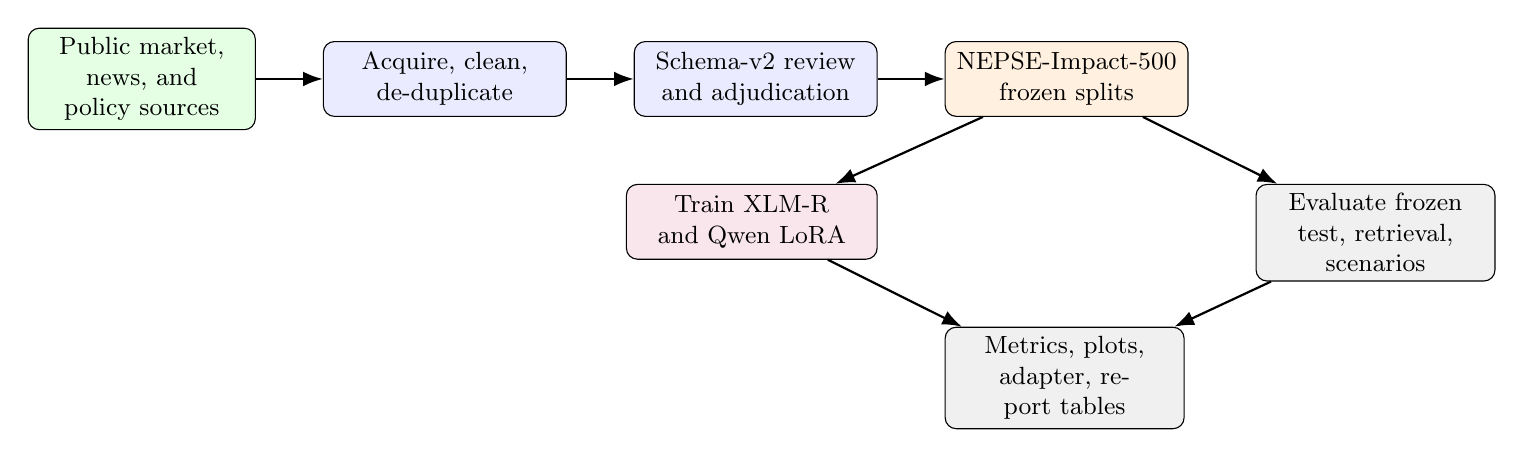
\begin{tikzpicture}[
    node distance=0.85cm and 0.85cm,
    every node/.style={font=\small},
    source/.style={draw, rounded corners, align=center, text width=2.65cm, minimum height=0.95cm, fill=green!10},
    process/.style={draw, rounded corners, align=center, text width=2.85cm, minimum height=0.95cm, fill=blue!8},
    store/.style={draw, rounded corners, align=center, text width=2.85cm, minimum height=0.95cm, fill=orange!12},
    model/.style={draw, rounded corners, align=center, text width=2.95cm, minimum height=0.95cm, fill=purple!10},
    output/.style={draw, rounded corners, align=center, text width=2.8cm, minimum height=0.95cm, fill=gray!12},
    arrow/.style={-{Latex[length=2.5mm]}, thick}
]
\node[source] (sources) {Public market, news, and policy sources};
\node[process, right=of sources] (acq) {Acquire, clean, de-duplicate};
\node[process, right=of acq] (review) {Schema-v2 review and adjudication};
\node[store, right=of review] (splits) {NEPSE-Impact-500 frozen splits};
\node[model, below left=of splits] (train) {Train XLM-R and Qwen LoRA};
\node[output, below right=of splits] (eval) {Evaluate frozen test, retrieval, scenarios};
\node[output, below right=of train] (artifacts) {Metrics, plots, adapter, report tables};

\draw[arrow] (sources) -- (acq);
\draw[arrow] (acq) -- (review);
\draw[arrow] (review) -- (splits);
\draw[arrow] (splits) -- (train);
\draw[arrow] (splits) -- (eval);
\draw[arrow] (train) -- (artifacts);
\draw[arrow] (eval) -- (artifacts);
\end{tikzpicture}
}%
\caption{Training and evaluation workflow.}
\label{fig:training-workflow}
\end{figure}

\begin{figure}[htbp]
\centering
\resizebox{\textwidth}{!}{%
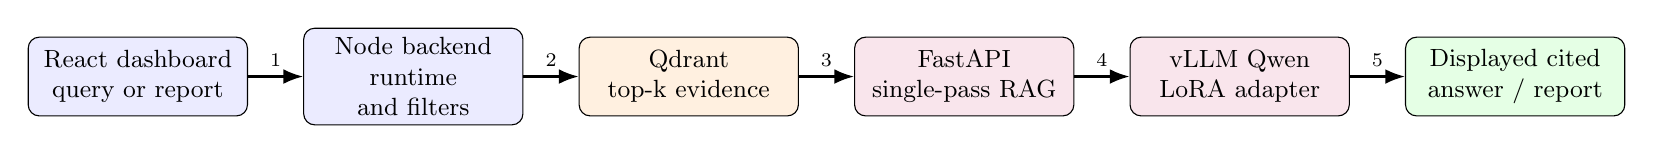
\begin{tikzpicture}[
    node distance=0.7cm,
    every node/.style={font=\small},
    flowstep/.style={draw, rounded corners, align=center, text width=2.55cm, minimum height=1.0cm, fill=blue!8},
    store/.style={draw, rounded corners, align=center, text width=2.55cm, minimum height=1.0cm, fill=orange!12},
    model/.style={draw, rounded corners, align=center, text width=2.55cm, minimum height=1.0cm, fill=purple!10},
    output/.style={draw, rounded corners, align=center, text width=2.55cm, minimum height=1.0cm, fill=green!10},
    arrow/.style={-{Latex[length=2.5mm]}, thick}
]
\node[flowstep] (ui) {React dashboard\\query or report};
\node[flowstep, right=of ui] (node) {Node backend\\runtime and filters};
\node[store, right=of node] (qdrant) {Qdrant\\top-k evidence};
\node[model, right=of qdrant] (agent) {FastAPI\\single-pass RAG};
\node[model, right=of agent] (vllm) {vLLM Qwen\\LoRA adapter};
\node[output, right=of vllm] (answer) {Displayed cited\\answer / report};

\draw[arrow] (ui) -- node[above, font=\scriptsize] {1} (node);
\draw[arrow] (node) -- node[above, font=\scriptsize] {2} (qdrant);
\draw[arrow] (qdrant) -- node[above, font=\scriptsize] {3} (agent);
\draw[arrow] (agent) -- node[above, font=\scriptsize] {4} (vllm);
\draw[arrow] (vllm) -- node[above, font=\scriptsize] {5} (answer);
\end{tikzpicture}
}%
\caption{Daily inference workflow.}
\label{fig:daily-inference}
\end{figure}

\section{Data Acquisition Method}
The data acquisition strategy follows the proposal's primary-and-fallback design. For market data, official NEPSE pages are preferred when a field is available in a stable form. ShareSansar and MeroLagani are used as fallback or corroborating sources for current values, listed securities, and historical index backfill. The collector records source provenance, selected source, missing fields, warnings, and conflicts rather than silently merging inconsistent values.

Financial news is collected from ShareSansar, OnlineKhabar Business, and Kathmandu Post Money. ShareSansar is collected through category-specific pagination across NEPSE news, public issues, allotments, dividends, financial analysis, listed shares, and stock-market coverage. OnlineKhabar collection uses paginated Business RSS pages and retrieves full article text when available. Kathmandu Post Money is included as a supplementary source because its historical pagination is limited. Articles shorter than 120 cleaned characters are rejected to avoid media stubs.

Regulatory documents are discovered from NRB and SEBON pages. The final system stores machine-readable text and extraction status, but OCR and legacy-font conversion are excluded from the final deliverable. This keeps the benchmark and RAG index grounded in text that can be inspected and cited.

\section{Data Pipeline and Storage Contract}
The latest final-report snapshot contains 224 historical market snapshots, 2,025 complete financial-news documents, 2,046 eligible documents, 350 active NEPSE symbols, and 2,038 Qdrant evidence chunks in the local MarketGyan collection. Historical market snapshots are marked partial when official breadth, leaders, or sector history fields are unavailable.

Operational storage is split across several contracts. \texttt{MarketSnapshot} stores daily index and turnover metrics, sectors, leaders, provenance, and warnings. \texttt{MarketDocument} stores article or regulatory-document metadata, cleaned text, content hash, source, language, companies, sectors, and extraction method. \texttt{MarketSecurity} stores the active symbol registry and aliases. \texttt{MarketLabel} stores immutable model inputs, generated candidates, numbered source sentences, token usage, errors, and adjudication state. \texttt{MarketAnnotation} stores independent reviewer annotations, and \texttt{MarketReaction} stores evaluation-only publication alignment and return windows.

\section{Benchmark Construction}
The first schema version produced a useful pilot but exposed a quality problem: some general-business stories were being forced into bullish, bearish, or neutral impact labels without a defensible NEPSE mechanism. That corpus was frozen as a pilot audit. Schema v2 then separated market relevance from potential impact, added a Nepal-market ontology, required numbered sentence evidence, and supported independent annotations and adjudication.

The final benchmark, NEPSE-Impact-500, contains 500 adjudicated rows:
\begin{itemize}[leftmargin=1.6em]
    \item 300 direct market-relevant records;
    \item 100 indirect sector or macro records;
    \item 100 hard-negative not-relevant records;
    \item 299 English, 200 Nepali, and 1 mixed-language record;
    \item 273 symbol-level records; and
    \item at least 20 records in each required core event category.
\end{itemize}
The approved JSONL was split into frozen train, validation, and test sets of 350, 75, and 75 rows using balanced duplicate grouping.

\section{Schema-v2 Curation and Structured Output Contract}
Each schema-v2 record preserves the source document, numbered sentences, immutable generated candidate, independent annotations, and final adjudicated gold label. The training export uses the gold label while retaining enough metadata to audit evidence and duplicate groups. The relevant compact JSONL shape is:

\begin{small}
\begin{verbatim}
{
  "id": "...",
  "title": "...",
  "sentences": [{"id": "S1", "text": "..."}],
  "source": {"name": "...", "url": "..."},
  "publishedAt": "...",
  "contentHash": "...",
  "duplicateGroupId": "...",
  "gold": {
    "relevance": "direct",
    "eventType": "earnings",
    "impactScope": "company",
    "impactDirection": "bullish",
    "impactHorizon": "short_term",
    "impactMechanism": "earnings_cash_flow",
    "sectors": ["Banking"],
    "symbols": ["NABIL"],
    "confidenceBand": "medium",
    "evidenceSentenceIds": ["S1"]
  }
}
\end{verbatim}
\end{small}

The compact model output intentionally excludes long rationales and report prose. The generator is asked to emit only the fields needed for classification and evidence selection:

\begin{small}
\begin{verbatim}
{
  "relevance": "direct | indirect | not_relevant",
  "eventType": "market_trading | earnings | regulation | ...",
  "impactScope": "market | sector | company | not_applicable",
  "impactDirection": "bullish | bearish | neutral | ...",
  "impactHorizon": "immediate | short_term | ...",
  "impactMechanism": "market_flow | earnings_cash_flow | ...",
  "sectors": ["..."],
  "symbols": ["..."],
  "confidenceBand": "low | medium | high",
  "evidenceSentenceIds": ["S1", "S3"]
}
\end{verbatim}
\end{small}

Validation rejects missing fields, unsupported enum values, unregistered symbols, sectors outside the taxonomy, relevant rows without defensible impact fields, not-relevant rows with inappropriate impact fields, and evidence IDs that are not present in the numbered source sentences. Duplicate groups remain in the same split so that near-duplicate article versions do not leak between train, validation, and test.

\section{Training Flow}
Training examples are generated as two-message chat records. The user message contains the document title and numbered source sentences; the assistant message contains the compact adjudicated JSON output. For XLM-R, title and excerpt are concatenated and used for supervised classification. For Qwen, the chat template is configured so the adapter learns the JSON response rather than prompt text. The frozen test split is never used for oversampling or prompt repair.

\section{Modeling}
The project evaluated a progression of models so that the final Qwen result could be interpreted against simpler baselines. Table \ref{tab:modeling-plan} summarizes the modeling roles.

\begin{table}[htbp]
\centering
\caption{Modeling roles used in MarketGyan.}
\label{tab:modeling-plan}
\small
\begin{tabularx}{\textwidth}{@{}L{0.25\textwidth}L{0.25\textwidth}Y@{}}
\toprule
Model path & Role & Reason for inclusion \\
\midrule
XLM-R relevance classifier & Multilingual supervised baseline & Tests whether a compact encoder can learn direct, indirect, and not-relevant classes from English and Nepali text. \\
XLM-R direction classifier & Supervised sentiment/impact baseline & Measures bullish, bearish, and neutral-or-uncertain direction on relevant records; neutral and uncertain are merged because standalone neutral has too few labels. \\
English-only FinBERT & Financial-domain sanity baseline & Tests financial sentiment transfer on the small English relevant subset, while exposing the limitation for Nepali text. \\
Base Qwen zero-shot and three-shot & Prompting ablation & Measures what the base instruction model can do before domain fine-tuning. \\
Qwen3-8B QLoRA & Diagnostic LLM adaptation & Exposed invalid JSON and grounding failures under 4-bit QLoRA. \\
Qwen3.5-9B BF16 LoRA targeted-v2 & Final trained candidate & Uses best-validation checkpoint selection and targeted oversampling for structured extraction. \\
\bottomrule
\end{tabularx}
\end{table}

The final adapter was trained on an A100 80GB profile with LoRA rank 32, max sequence length 2,048, batch size 4, gradient accumulation 2, learning rate \(2 \times 10^{-5}\), and best-validation checkpoint selection. The targeted-v2 oversampling profile expanded the 350 training rows to 922 weighted examples using only the frozen train split, with row weight capped at 8.

\section{Runtime Design}
The initial multi-agent prompt design was replaced for live use because it exceeded vLLM context windows even after increasing context length to 16k tokens. The final application path is a single-pass RAG agent. It retrieves compact evidence rows from Qdrant through the Node backend, sends bounded evidence and market context to the served Qwen3.5-9B adapter, asks the model to choose evidence indexes and draft a response, and then materializes citations from retrieved rows. This design keeps URLs, excerpts, content hashes, sentence IDs, and expanded sentence text under deterministic system control.

\begin{table}[htbp]
\centering
\caption{Runtime component responsibilities.}
\label{tab:runtime-design}
\small
\begin{tabularx}{\textwidth}{@{}L{0.28\textwidth}Y@{}}
\toprule
Component & Responsibility \\
\midrule
React dashboard & User-facing overview, Ask MarketGyan, Evidence Search, Reports, System, and validation views. \\
Node backend & Public API, retrieval endpoint, runtime status, report persistence, local report-generation guard, scheduler, and newsletter integration. \\
Qdrant & Sentence-level finance evidence chunks with source URL, title, source, content hash, sentence IDs, language, symbols, sectors, and tags. \\
FastAPI agent & Single-pass RAG orchestration, generator call, citation materialization, disclaimer and safety checks. \\
Lightning vLLM & OpenAI-compatible serving for \texttt{Qwen/Qwen3.5-9B} plus the \texttt{marketgyan-qwen35-9b-targeted-v2} LoRA adapter. \\
Evaluation harness & Frozen model scoring, constrained inference scoring, retrieval export/label scoring, and scenario checks. \\
\bottomrule
\end{tabularx}
\end{table}

\chapter{System Requirement Specification}

\section{Functional Requirements}
The final prototype implements the following proposal-aligned requirements:
\begin{itemize}[leftmargin=1.6em]
    \item ingest and update finance-specific market data and articles;
    \item store market documents, snapshots, labels, reports, and security aliases;
    \item index sentence-level evidence in a vector database;
    \item fine-tune and evaluate supervised and instruction-model baselines;
    \item serve the trained Qwen adapter through an OpenAI-compatible endpoint;
    \item answer finance questions with visible citations and disclaimer text;
    \item generate local daily market reports with source provenance; and
    \item maintain scenario, retrieval, and frozen-test evaluation artifacts.
\end{itemize}

\section{Non-Functional Requirements}
The system must be reproducible, citation-aware, and fail-closed. Model results are measured on frozen train/validation/test splits. Public answers must include disclaimers and must not provide buy or sell advice. Citation objects must include source title, URL, excerpt, chunk ID, content hash, sentence IDs, and expanded sentence text when available. Report generation remains loopback/protected during the demo because it writes archived report records.

\section{Resource Requirements}
\begin{table}[H]
\centering
\caption{Final resource requirements and actual runtime choices.}
\label{tab:resource-requirements}
\small
\begin{tabularx}{\textwidth}{@{}L{0.26\textwidth}Y@{}}
\toprule
Category & Requirement / actual choice \\
\midrule
Local development & macOS laptop with Node.js, Python, MongoDB, Docker, and enough storage for article data, model artifacts, and generated report outputs. \\
Backend and frontend & Existing Khabar AI stack: React, Node.js, Express, MongoDB, Qdrant, Node-Cron, Nodemailer, and Python/FastAPI. \\
Training hardware & A100 80GB GPU was used for the final Qwen3.5-9B BF16 LoRA run; XLM-R training uses standard transformer fine-tuning resources. \\
Inference hardware & Lightning AI Studio with vLLM was used for the served Qwen adapter; A100 40GB is sufficient for proposal testing when context length and batch size are controlled, while A100 80GB is safer. \\
Data resources & NEPSE market summaries, ShareSansar and other finance-news sources, selected NRB/SEBON machine-readable documents, and the adjudicated NEPSE-Impact-500 JSONL benchmark. \\
\bottomrule
\end{tabularx}
\end{table}

\section{XLM-R Training Configuration}
\begin{table}[H]
\centering
\caption{Implemented XLM-R baseline training configuration.}
\label{tab:xlmr-training-config}
\small
\begin{tabularx}{\textwidth}{@{}L{0.32\textwidth}Y@{}}
\toprule
Item & Configuration \\
\midrule
Base model & \texttt{xlm-roberta-base} \\
Input & Concatenated title and excerpt \\
Maximum input length & 512 tokens \\
Train / evaluation batch size & 8 / 16 \\
Learning rate & \(2 \times 10^{-5}\) \\
Epochs & 8 maximum \\
Weight decay & 0.01 \\
Tasks & Relevance on all records; direction on relevant records only (neutral and uncertain merged) \\
Imbalance handling & Effective-number class weights with count-driven minority oversampling \\
Selection metric & Validation macro-F1 \\
Early stopping & Patience of 2 epochs \\
Artifacts & Model, tokenizer, predictions, metrics JSON, and result plots \\
\bottomrule
\end{tabularx}
\end{table}

\section{Qwen3.5-9B Training Configuration}
\begin{table}[H]
\centering
\caption{Final Qwen3.5-9B targeted-v2 BF16 LoRA training configuration.}
\label{tab:qwen-training-config}
\small
\begin{tabularx}{\textwidth}{@{}L{0.32\textwidth}Y@{}}
\toprule
Item & Configuration \\
\midrule
Base model & \texttt{Qwen/Qwen3.5-9B} \\
Precision / quantization & BF16 LoRA, no 4-bit loading for the official candidate \\
Maximum sequence length & 2,048 tokens \\
Maximum generation tokens & 256 \\
LoRA rank / alpha / dropout & 32 / 64 / 0.05 \\
Train / evaluation batch size & 4 / 4 per device \\
Gradient accumulation & 2 steps \\
Epochs & 3 \\
Learning rate & \(2 \times 10^{-5}\) \\
Optimizer & \texttt{paged\_adamw\_8bit} \\
Evaluation / save interval & Every 10 steps \\
Best checkpoint & Loaded by validation loss with \texttt{greater\_is\_better=false} \\
Oversampling & \texttt{targeted\_v2}; 350 train rows expanded to 922 weighted examples; cap 8 \\
Output & \begin{tabular}[t]{@{}l@{}}\texttt{marketgyan-qwen35-9b-a100-80gb-}\\\texttt{bf16-lora-targeted-v2}\end{tabular} \\
\bottomrule
\end{tabularx}
\end{table}

\chapter{Implementation}

\section{Backend Data Services}
MarketGyan is implemented as an extension of the existing Khabar AI backend rather than as a separate standalone server. The Node backend manages market-data ingestion, article records, label/review tooling, runtime status, protected report generation, report persistence, scheduler execution, and newsletter integration. MongoDB stores article, market snapshot, market document, label, annotation, security, and report records. Upserts use stable source URLs and content hashes so that rerunning collectors does not duplicate unchanged documents.

\section{Annotation and Validation Tools}
The data-curation implementation supports three stages: generated candidate creation, independent review, and adjudication. The generated candidate is immutable and used for acceptance/edit-rate analysis. Reviewer edits are stored separately, and only adjudicated gold records enter the v2 export. The validator checks schema version, ontology enums, relevance consistency, sector taxonomy, registered symbols, source metadata, duplicate group IDs, date fields, and sentence-ID grounding. Pending, excluded, v1, and non-adjudicated rows are blocked from training export.

\section{Vector Indexing and Retrieval}
Qdrant stores finance-specific evidence chunks. Each point contains chunk text and metadata such as MongoDB document ID, chunk ID, title, canonical URL, source, publication date, language, document type, sectors, symbols, tags, content hash, sentence IDs, and expanded sentence text. The indexer is idempotent: unchanged content keeps stable point identifiers, while changed content replaces stale points. Search supports query text plus filters for date, sector, source, language, and document type. The final local collection used for the demo contains 2,038 points.

\section{Model Serving}
Model training and evaluation are implemented in the MarketGyan ML workspace. The XLM-R baseline notebook trains relevance and direction classifiers and exports metrics, predictions, and plots. The Qwen notebook/script path loads the selected profile environment, builds chat-formatted JSON examples, applies optional oversampling, trains the LoRA adapter, saves the best validation checkpoint, exports metrics, writes a training profile, and generates deep error slices. The final adapter is served through Lightning AI using vLLM's OpenAI-compatible endpoint. The active runtime candidate is \texttt{Qwen/Qwen3.5-9B} with the LoRA adapter \texttt{marketgyan-qwen35-9b-targeted-v2}. Direct unconstrained prompting is diagnostic only because it can emit reasoning text before JSON. JSON Schema constrained decoding is the correct model-only structured inference path, while the single-pass RAG agent is the correct application path.

\section{Single-Pass Agent and Reports}
The FastAPI agent receives a query or report request, calls the protected Node retrieval endpoint, constructs compact evidence rows, and sends bounded evidence plus market context to the served Qwen adapter. The model returns answer text and selected evidence indexes. The agent then materializes citations from retrieved rows instead of trusting the model to invent URLs or sentence IDs. For reports, the Node backend persists the generated report, citations, sector analysis, and report status. Report generation is local-only in the demo environment because it writes archived records.

\section{Frontend Demonstration}
The React MarketGyan dashboard contains Overview, Ask MarketGyan, Evidence Search, Reports, System, and validation views. The Overview tab shows market snapshot and runtime readiness. Ask MarketGyan sends a grounded query to the backend/agent path and renders disclaimer text, answer text, citations, sentence IDs, and expanded sentence evidence. Evidence Search allows direct retrieval inspection. Reports can force local generation for the latest available snapshot date and display the archived report with sector analysis and evidence citations. The System tab exposes query, review, local report generation, agent-token, Qdrant, snapshot, and latest-report status checks for demo readiness.

\section{Safety and Fail-Closed Behavior}
MarketGyan is informational only. The agent and report paths require disclaimers and reject direct buy or sell advice. If retrieval is weak, if source fields are missing, if the agent token is not configured, or if citation validation fails, the runtime should fail closed rather than publish uncited analysis. This behavior is important because the model content metrics and retrieval quality are not strong enough to justify unsupported generated claims.

\chapter{Results and Evaluation}

\section{Baseline Model Results}
The first supervised baseline used XLM-R because it supports both English and Nepali text. It was trained separately for relevance and direction. The relevance classifier uses all 75 frozen test rows, while the direction classifier is evaluated on the 60 relevant test rows. An English-only FinBERT run was also evaluated as a small financial-domain variant on the English relevant subset. Table \ref{tab:baseline-results} summarizes these baseline outputs.

\begin{table}[htbp]
\centering
\caption{XLM-R and FinBERT baseline results.}
\label{tab:baseline-results}
\small
\begin{tabularx}{\textwidth}{@{}L{0.29\textwidth}rrrrY@{}}
\toprule
Model / task & Accuracy & Macro-F1 & Errors & Support & Notes \\
\midrule
XLM-R relevance & 0.813 & 0.743 & 14 & 75 & Direct / indirect / not-relevant classification. \\
XLM-R direction & 0.567 & 0.568 & 26 & 60 & Bullish / bearish / neutral-or-uncertain (merged) on relevant records. \\
English-only FinBERT direction & 0.889 & 0.616 & 3 & 14 & Small English relevant subset; useful only as a sanity baseline. \\
\bottomrule
\end{tabularx}
\end{table}

\begin{figure}[htbp]
\centering
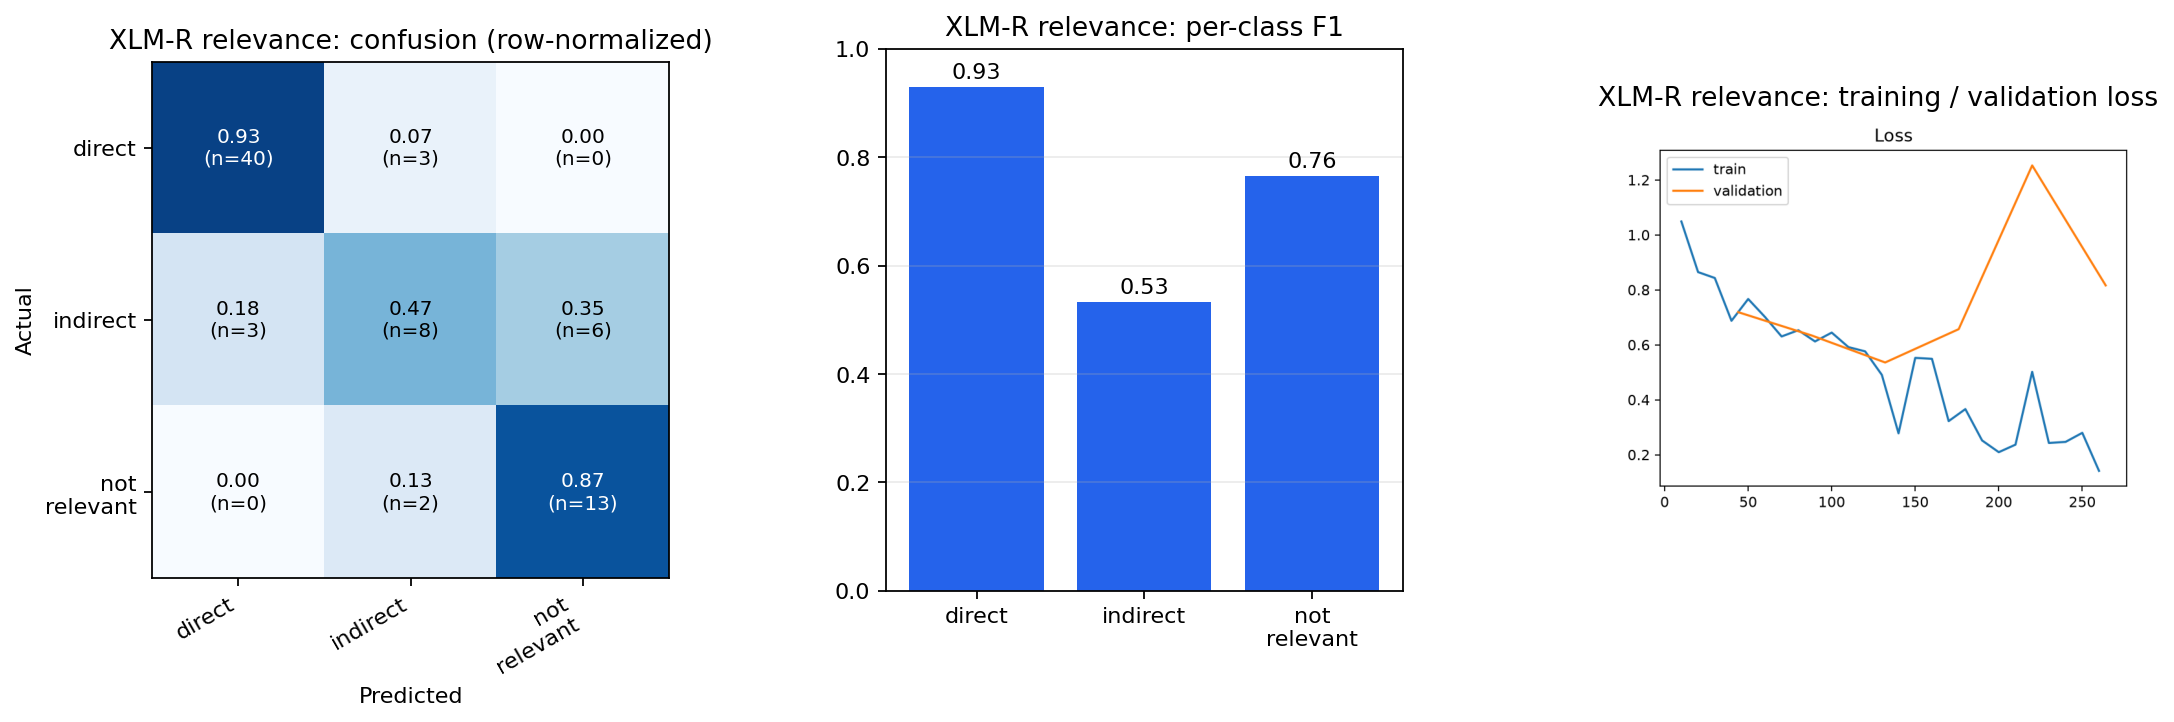
\includegraphics[width=\textwidth]{images/xlmr-relevance-combined.png}
\caption{XLM-R relevance baseline on the frozen test split: row-normalized confusion matrix, per-class F1, and the training/validation loss curve.}
\label{fig:xlmr-relevance}
\end{figure}

\begin{figure}[htbp]
\centering
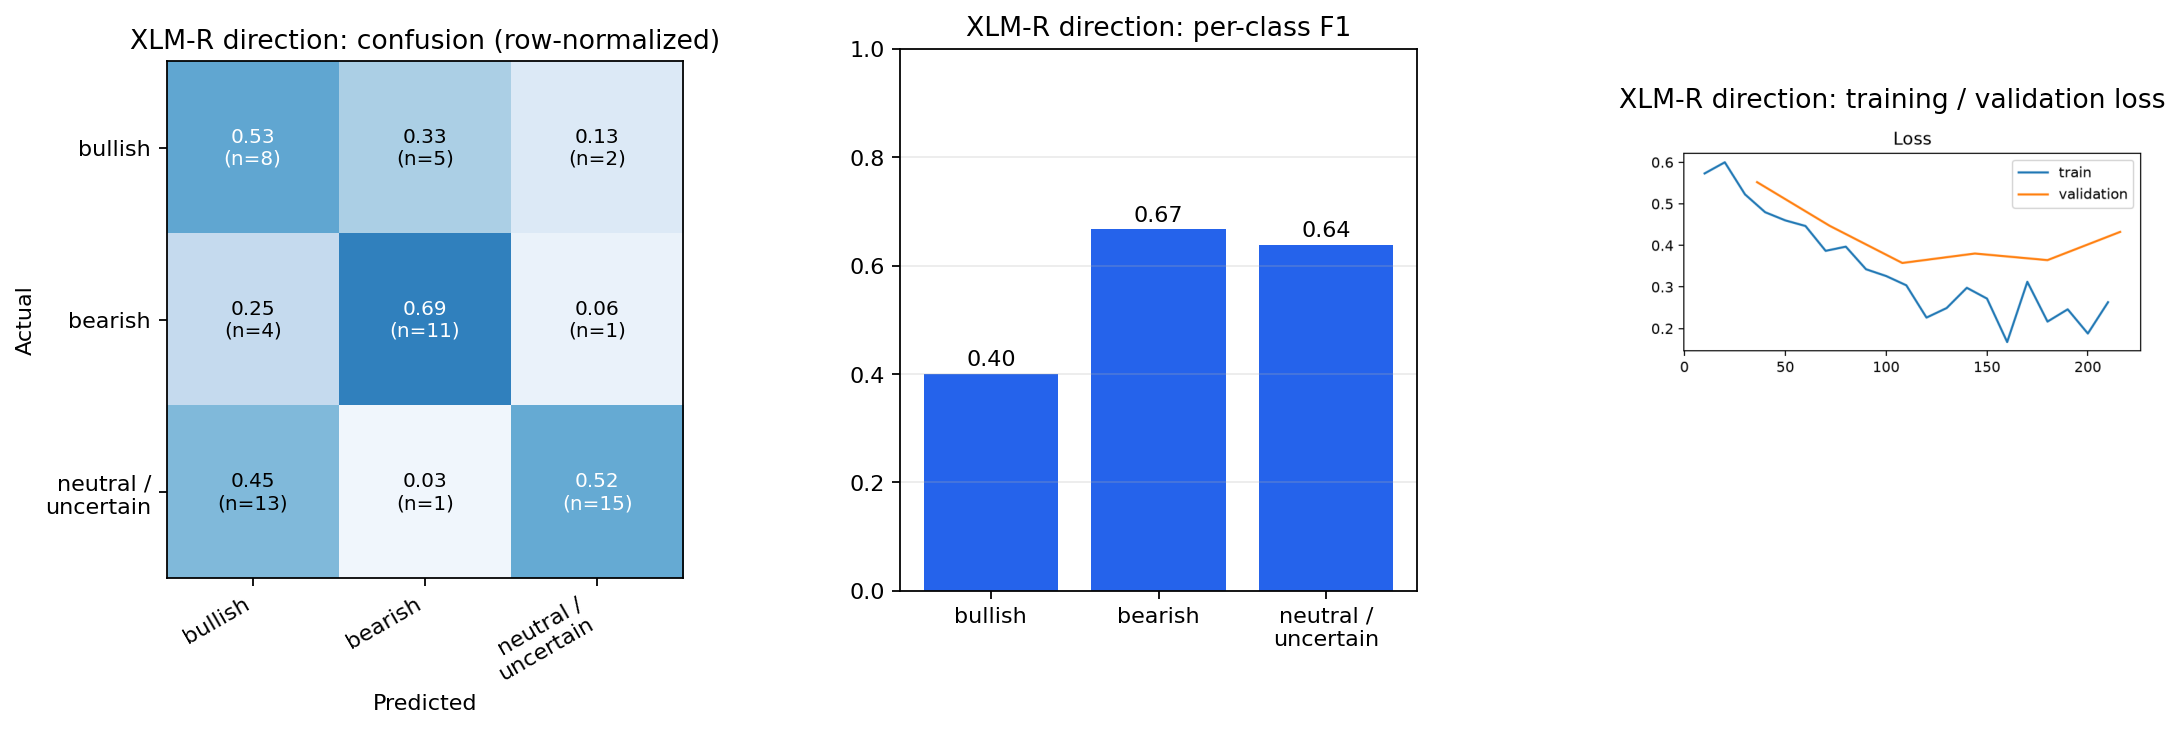
\includegraphics[width=\textwidth]{images/xlmr-direction-combined.png}
\caption{XLM-R direction baseline (merged neutral-or-uncertain target) on the relevant frozen-test rows: row-normalized confusion matrix, per-class F1, and the training/validation loss curve. The merged target avoids the standalone neutral class, which has too few labels to learn reliably.}
\label{fig:xlmr-direction}
\end{figure}

XLM-R provides a reliable multilingual classifier baseline, but it does not generate structured evidence-grounded outputs. The relevance model is strong on the \texttt{direct} and \texttt{not\_relevant} classes and weaker on the fuzzier \texttt{indirect} class. For direction, merging the adjacent neutral and uncertain labels into one non-directional class avoids a class that the corpus cannot yet support, and the resulting model separates bullish, bearish, and neutral-or-uncertain movement with no dead class. FinBERT shows that financial-domain adaptation helps on English sentiment examples, but its small support and English-only scope make it insufficient for the bilingual MarketGyan task.

\section{Qwen Model-Only Benchmark}
Table \ref{tab:modelresults} summarizes the frozen test-set result for the final Qwen3.5-9B targeted-v2 adapter compared with the previous A100 baseline.

\begin{table}[htbp]
\centering
\caption{Strict frozen-test comparison for Qwen3.5-9B A100 runs.}
\label{tab:modelresults}
\small
\begin{tabular}{@{}lrrr@{}}
\toprule
Metric & Baseline & Targeted-v2 & Change \\
\midrule
Structured-output validity & 0.960 & 1.000 & +0.040 \\
Evidence grounding & 0.987 & 1.000 & +0.013 \\
Invalid outputs & 3 & 0 & -3 \\
Relevance macro-F1 & 0.735 & 0.796 & +0.061 \\
Nepali relevance accuracy & 0.667 & 0.788 & +0.121 \\
Event macro-F1 & 0.597 & 0.633 & +0.036 \\
Direction macro-F1 & 0.582 & 0.575 & -0.007 \\
Neutral direction recall & 0.000 & 0.000 & 0.000 \\
Sector micro-F1 & 0.759 & 0.677 & -0.082 \\
Symbol micro-F1 & 0.815 & 0.793 & -0.022 \\
Evidence sentence micro-F1 & 0.765 & 0.736 & -0.028 \\
\bottomrule
\end{tabular}
\end{table}

The final adapter passes the structural gate and improves relevance, especially for Nepali records. It does not pass the full content gate because event macro-F1 remains below 0.65, direction macro-F1 remains below 0.65, neutral recall is zero, and set-valued sector, symbol, and evidence metrics remain below target.

\begin{figure}[htbp]
\centering
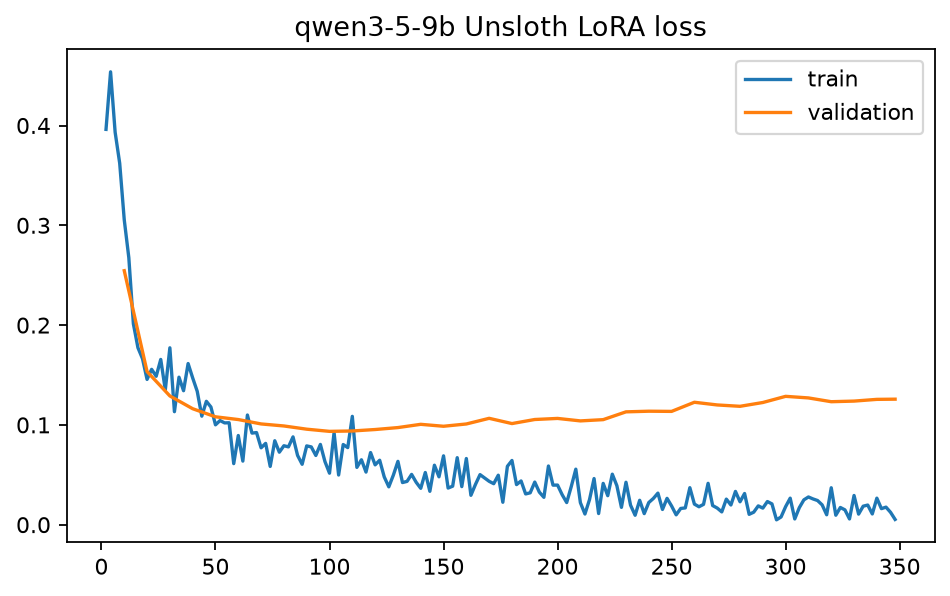
\includegraphics[width=0.88\textwidth]{images/qwen-targeted-v2-loss.png}
\caption{Qwen3.5-9B targeted-v2 training and evaluation loss curve from the latest A100 output artifact.}
\label{fig:qwen-loss}
\end{figure}

\begin{figure}[htbp]
\centering
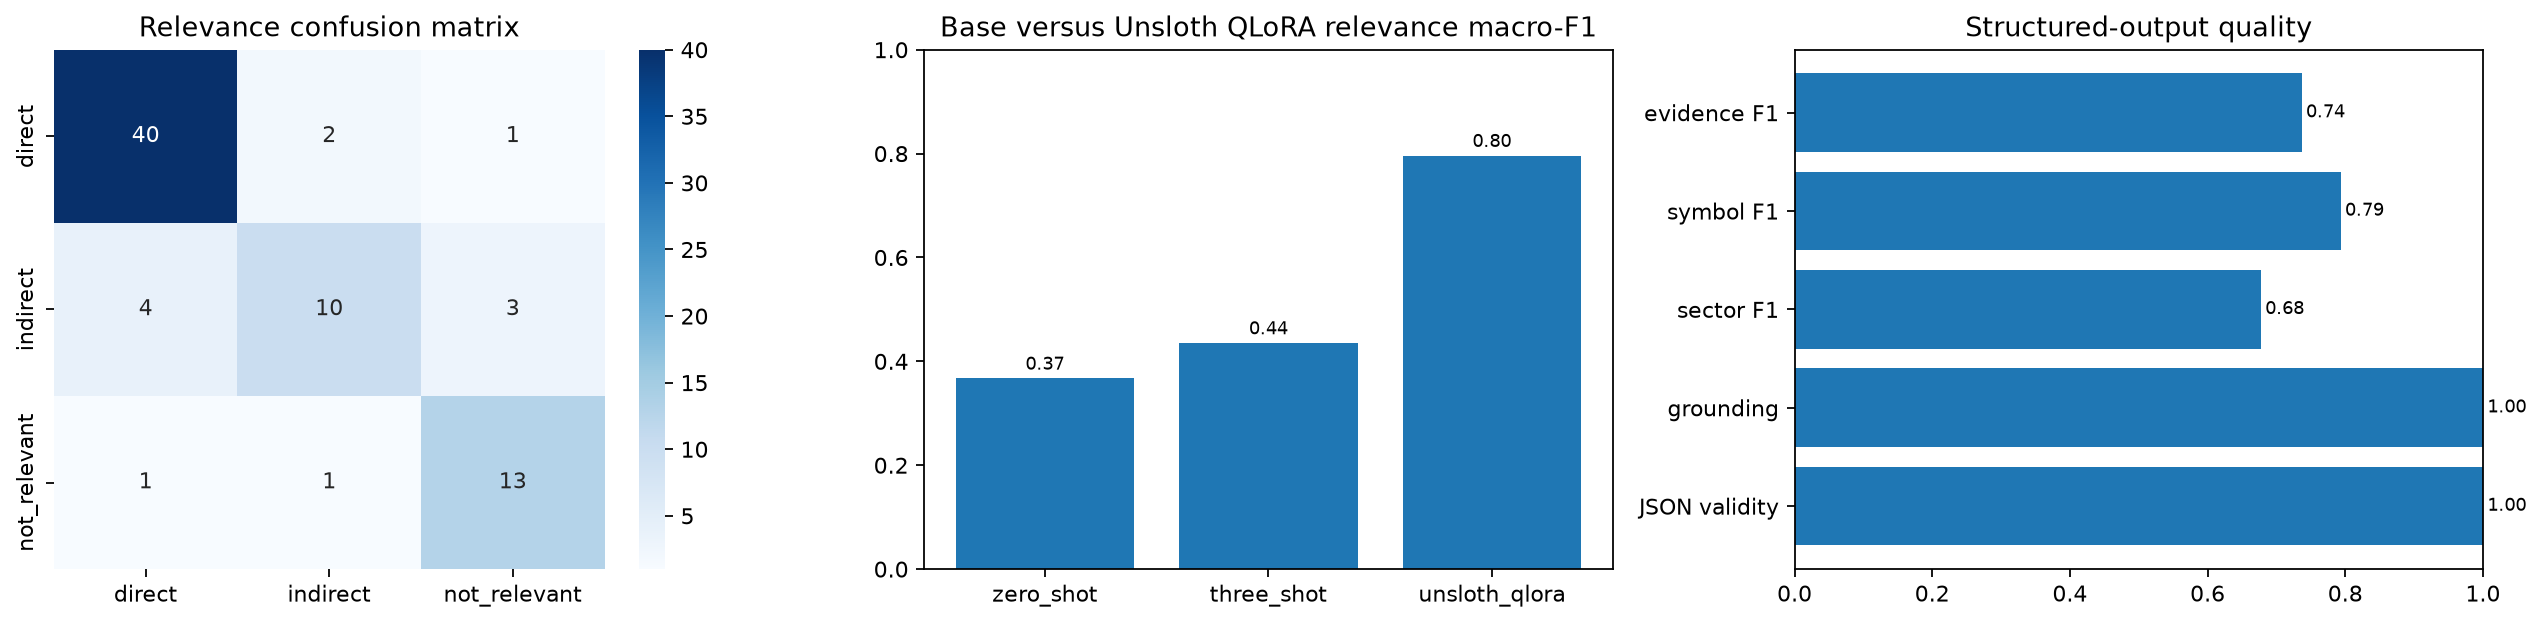
\includegraphics[width=0.88\textwidth]{images/qwen-targeted-v2-test-results.png}
\caption{Qwen3.5-9B targeted-v2 frozen-test summary plot exported with the final adapter artifact.}
\label{fig:qwen-test-results}
\end{figure}

\section{Qwen Prompting and Fine-Tuning Ablation}
The Qwen artifact contains zero-shot, three-shot, and fine-tuned adapter predictions on the same frozen 75-row test split. This makes it possible to isolate the effect of prompting versus fine-tuning. Table \ref{tab:qwen-ablation} shows that base prompting can sometimes classify event type, but it does not reliably produce valid grounded JSON. Fine-tuning is the main reason strict validity and grounding reach 1.000 and set-field extraction becomes usable.

\begin{table}[htbp]
\centering
\caption{Qwen zero-shot, few-shot, and fine-tuned ablation on the frozen test split.}
\label{tab:qwen-ablation}
\scriptsize
\resizebox{\textwidth}{!}{%
\begin{tabular}{@{}lrrrrrrrrr@{}}
\toprule
Qwen condition & Validity & Grounding & Invalid & Rel. Acc. & Rel. Macro-F1 & Event Macro-F1 & Dir. Macro-F1 & Sector F1 & Symbol F1 \\
\midrule
Base zero-shot & 0.000 & 0.000 & 75 & 0.627 & 0.367 & 0.566 & 0.506 & 0.013 & 0.444 \\
Base three-shot & 0.987 & 0.987 & 1 & 0.640 & 0.435 & 0.532 & 0.502 & 0.086 & 0.380 \\
Qwen3.5-9B LoRA targeted-v2 & 1.000 & 1.000 & 0 & 0.840 & 0.796 & 0.633 & 0.575 & 0.677 & 0.793 \\
\bottomrule
\end{tabular}
}%
\end{table}

\begin{table}[htbp]
\centering
\caption{Qwen evidence-selection ablation.}
\label{tab:qwen-evidence-ablation}
\small
\begin{tabularx}{\textwidth}{@{}L{0.46\textwidth}rrr@{}}
\toprule
Qwen condition & Evidence F1 & Direction acc. & Event acc. \\
\midrule
Base zero-shot & 0.000 & 0.567 & 0.767 \\
Base three-shot & 0.599 & 0.550 & 0.667 \\
Qwen3.5-9B LoRA targeted-v2 & 0.736 & 0.700 & 0.750 \\
\bottomrule
\end{tabularx}
\end{table}

The ablation shows three important patterns. First, zero-shot base Qwen often emits numeric evidence IDs or malformed outputs, producing zero strict validity. Second, three-shot prompting greatly improves structural behavior but does not improve relevance macro-F1 enough. Third, the targeted-v2 fine-tune improves relevance, evidence selection, sector selection, and symbol selection, but still fails to learn the rare neutral direction class.

\section{Constrained Runtime Inference}
The frozen adapter was also tested through vLLM JSON Schema constrained decoding on the unchanged 75-row test split. Structured validity and evidence grounding remained above the 0.95 gate at 0.987 each. Relevance macro-F1 improved to 0.819, but event, sector, symbol, and evidence metrics declined. This confirms that constrained decoding is useful for schema safety but is not a substitute for better content modeling or retrieval.

\begin{table}[htbp]
\centering
\caption{Model-only adapter output versus vLLM JSON Schema constrained inference.}
\label{tab:constrained-inference}
\small
\begin{tabular}{@{}lrrr@{}}
\toprule
Metric & Adapter output & Constrained vLLM & Change \\
\midrule
Structured-output validity & 1.000 & 0.987 & -0.013 \\
Evidence grounding & 1.000 & 0.987 & -0.013 \\
Invalid outputs & 0 & 1 & +1 \\
Relevance macro-F1 & 0.796 & 0.819 & +0.023 \\
Event macro-F1 & 0.633 & 0.604 & -0.029 \\
Direction macro-F1 & 0.575 & 0.585 & +0.010 \\
Sector micro-F1 & 0.677 & 0.643 & -0.034 \\
Symbol micro-F1 & 0.793 & 0.709 & -0.084 \\
Evidence sentence micro-F1 & 0.736 & 0.704 & -0.032 \\
\bottomrule
\end{tabular}
\end{table}

\chapter{Limitations and Future Work}

\section{Limitations}
\begin{itemize}[leftmargin=1.6em]
    \item NEPSE-Impact-500 is useful but small; rare event classes and the neutral direction class are still under-covered, so neutral direction cannot yet be learned as a standalone label.
    \item Historical market snapshots are partial and do not contain complete official fields for every date.
    \item Set-valued sector, symbol, and evidence-sentence extraction show a recall gap: the model selects valid items but often selects too few.
    \item Lightning-hosted vLLM is suitable for demonstration but is not a production deployment architecture by itself.
\end{itemize}

\section{Future Work}
\begin{enumerate}[leftmargin=1.7em]
    \item expand and adjudicate more neutral, sector-industry, regulation, and credit-financing hard cases so the direction task can move beyond the merged neutral-or-uncertain target;
    \item improve set-valued sector, symbol, and evidence recall through clearer selection rules and constrained post-processing;
    \item complete independent second annotation and report inter-annotator agreement metrics; and
    \item keep JSON Schema constrained inference and the single-pass RAG path as the production candidates while hardening deployment beyond the demo environment.
\end{enumerate}

\chapter{Conclusion}
MarketGyan successfully extends Khabar AI into a Nepal-specific financial NLP research prototype. It contributes NEPSE-Impact-500, a bilingual evidence-grounded benchmark; a Qwen3.5-9B targeted-v2 LoRA adapter; a finance-specific Qdrant evidence index; a single-pass RAG agent; and a React dashboard capable of demonstrating grounded query and report generation. The final model passes strict structure and grounding gates. However, several content metrics, including neutral direction recall and set-valued sector, symbol, and evidence recall, remain below the proposal gates. The project should therefore be submitted as a strong demo-ready research prototype with clear remaining work, not as a deployable financial advisory product.

\appendix
\chapter{Demo Screenshots}

The screenshots in this appendix are extracted from the final local Qwen demo
recording included with this submission in the \texttt{demo-recording}
directory as \texttt{marketgyan-qwen-demo.mp4}.
They document the frontend path used for the final smoke test: overview,
Ask MarketGyan, generated answer with evidence, and report generation.

\begin{figure}[htbp]
\centering
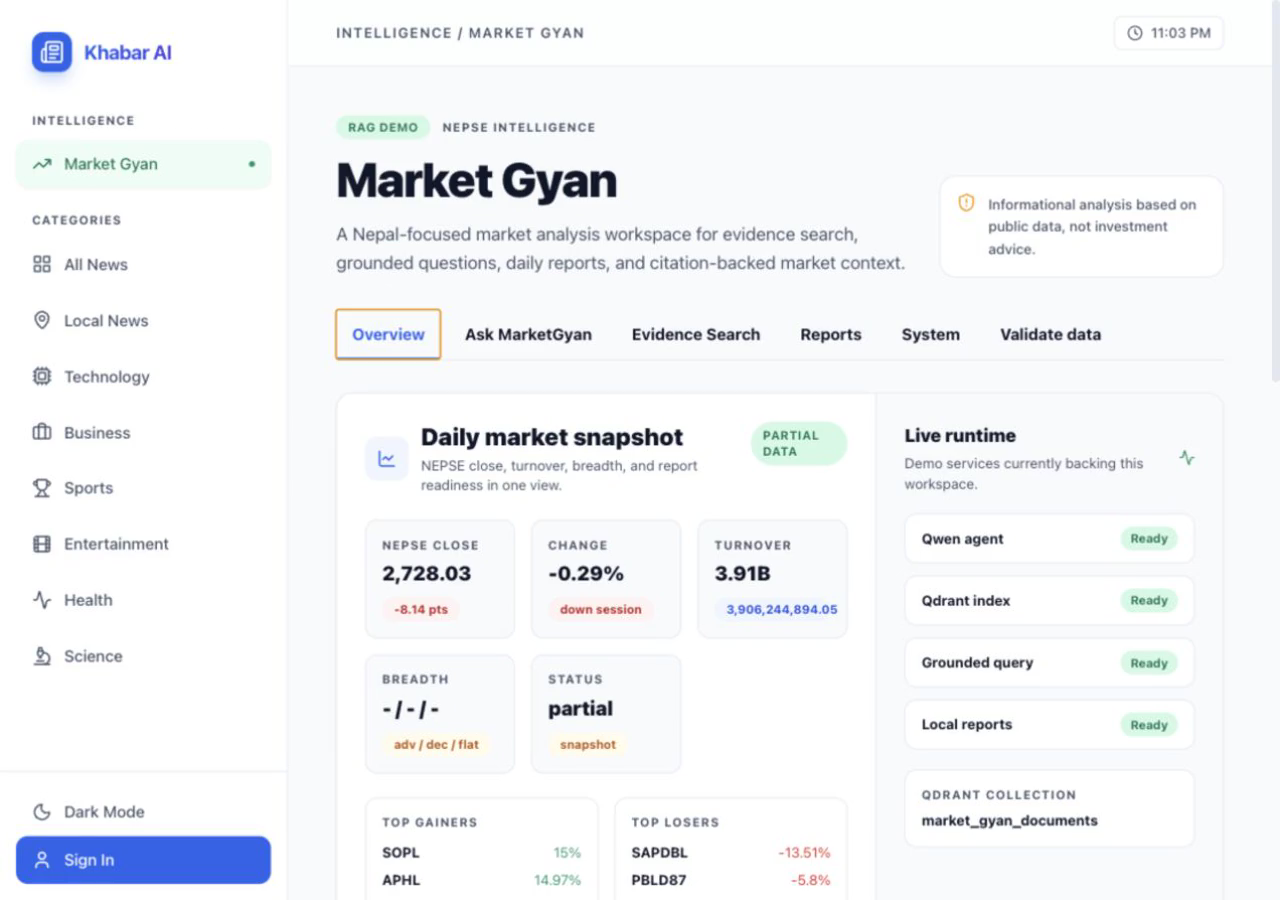
\includegraphics[width=\textwidth]{images/demo-2s.png}
\caption{MarketGyan overview tab showing market snapshot, live runtime checks, and Qdrant collection status.}
\label{fig:appendix-overview}
\end{figure}

\begin{figure}[htbp]
\centering
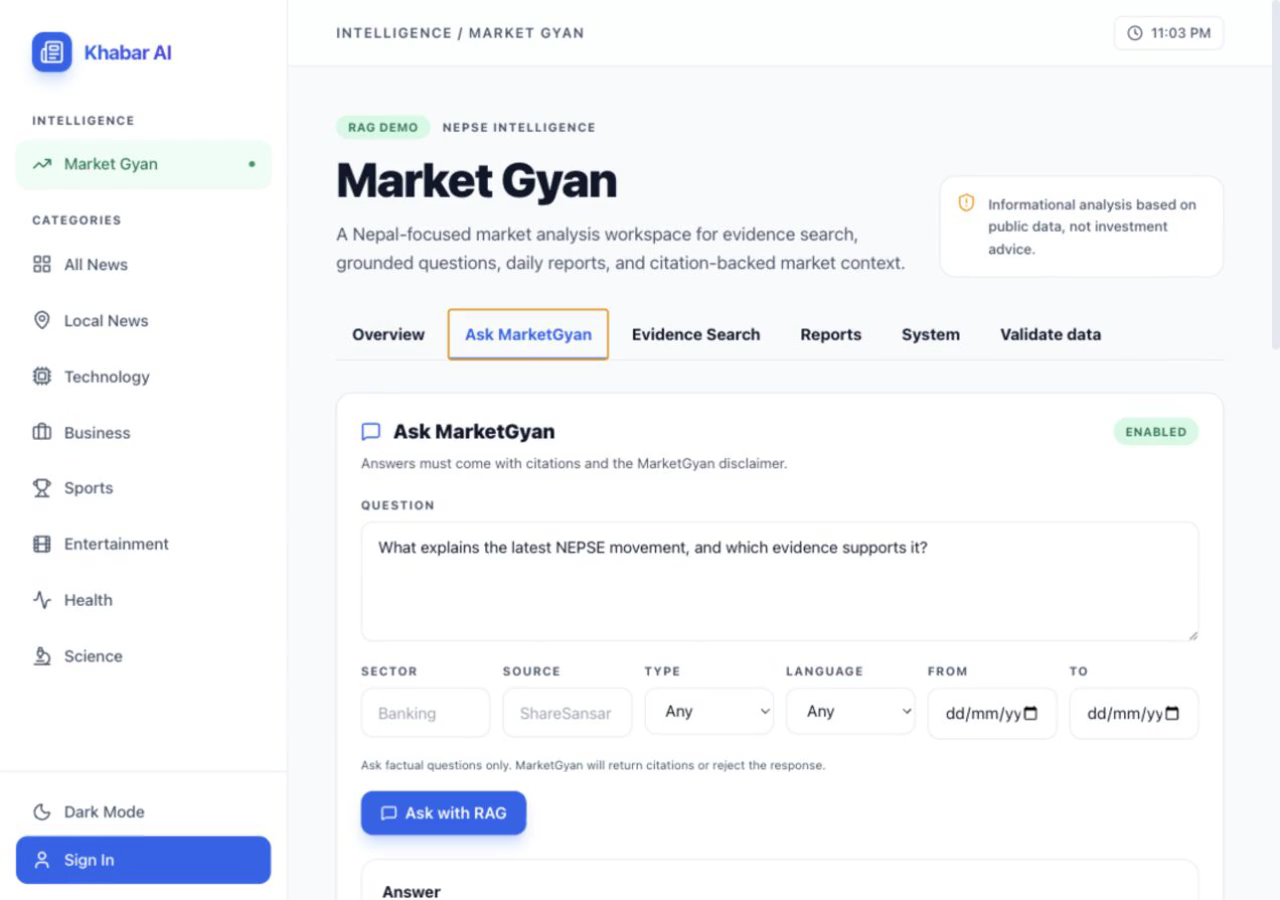
\includegraphics[width=\textwidth]{images/demo-8s.png}
\caption{Ask MarketGyan tab with a proposal-style market query form.}
\label{fig:appendix-ask}
\end{figure}

\begin{figure}[htbp]
\centering
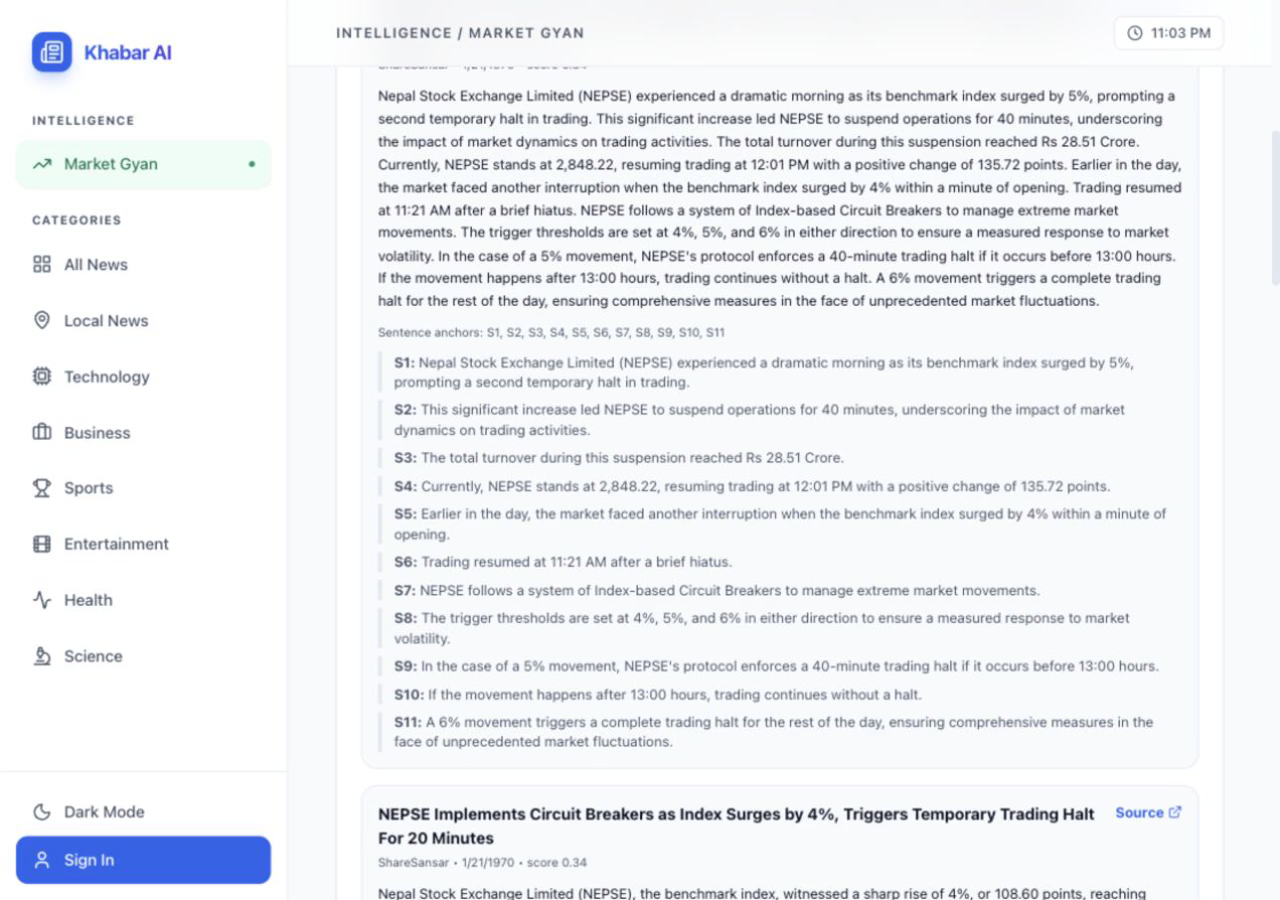
\includegraphics[width=\textwidth]{images/demo-14s.png}
\caption{Generated Qwen answer with disclaimer, sentence-grounded citations, and source evidence.}
\label{fig:appendix-answer}
\end{figure}

\begin{figure}[htbp]
\centering
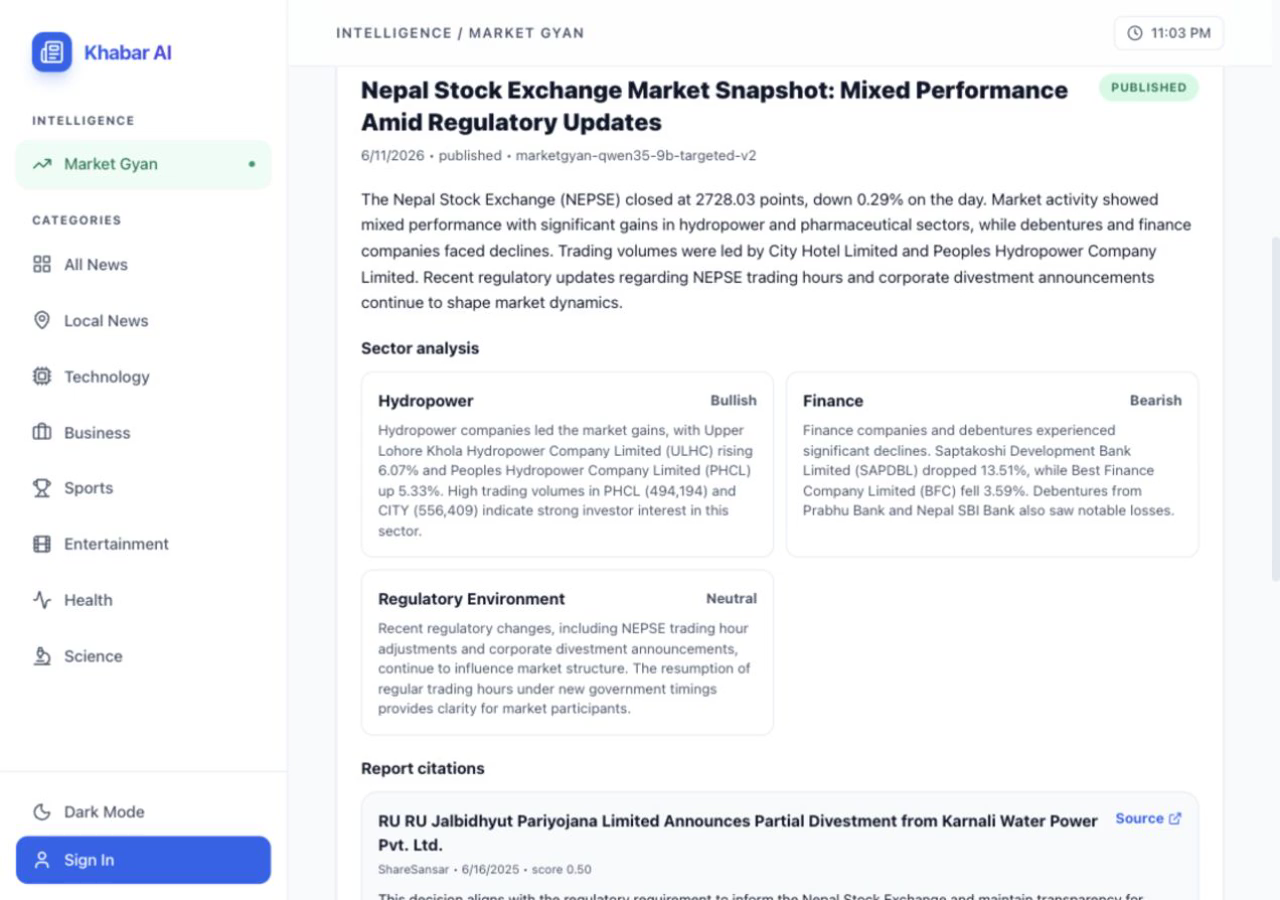
\includegraphics[width=\textwidth]{images/demo-21s.png}
\caption{Published MarketGyan report with headline, market summary, sector analysis, and report citations.}
\label{fig:appendix-report}
\end{figure}

\begingroup
\sloppy
\begin{thebibliography}{99}

\bibitem{araci2019finbert}
D. Araci, ``FinBERT: Financial Sentiment Analysis with Pre-trained Language Models,'' arXiv preprint arXiv:1908.10063, 2019.

\bibitem{yang2023fingpt}
H. Yang et al., ``FinGPT: Open-Source Financial Large Language Models,'' arXiv preprint arXiv:2306.06031, 2023.

\bibitem{lee2024finllms}
J. Lee, N. Stevens, S. C. Han, and M. Song, ``A Survey of Large Language Models in Finance,'' \emph{Neural Computing and Applications}, 2024.

\bibitem{bhatia2024fintral}
G. Bhatia et al., ``FinTral: A Family of GPT-4 Level Multimodal Financial Large Language Models,'' arXiv preprint arXiv:2402.10986, 2024.

\bibitem{timilsina2022}
S. Timilsina, M. Gautam, and B. Bhattarai, ``NepBERTa: Nepali Language Model Trained in a Large Corpus,'' in \emph{Proceedings of AACL-IJCNLP}, 2022, pp. 273--284.

\bibitem{subedi2024}
B. Subedi, S. Regmi, B. K. Bal, and P. Acharya, ``Exploring the Potential of Large Language Models for Low-resource Languages: A Study on Named-Entity Recognition and Part-of-Speech Tagging for Nepali Language,'' in \emph{LREC-COLING}, 2024, pp. 6974--6979.

\bibitem{thapa2025}
P. Thapa, J. Nyachhyon, M. Sharma, and B. K. Bal, ``Development of Pre-Trained Transformer-based Models for the Nepali Language,'' in \emph{CHiPSAL}, 2025, pp. 9--19.

\bibitem{hu2021lora}
E. J. Hu et al., ``LoRA: Low-Rank Adaptation of Large Language Models,'' in \emph{International Conference on Learning Representations}, 2022.

\bibitem{dettmers2023qlora}
T. Dettmers, A. Pagnoni, A. Holtzman, and L. Zettlemoyer, ``QLoRA: Efficient Finetuning of Quantized LLMs,'' in \emph{Advances in Neural Information Processing Systems}, vol. 36, 2023.

\bibitem{lewis2020rag}
P. Lewis et al., ``Retrieval-Augmented Generation for Knowledge-Intensive NLP Tasks,'' in \emph{Advances in Neural Information Processing Systems}, vol. 33, 2020, pp. 9459--9474.

\bibitem{gao2023alce}
T. Gao, H. Yen, J. Yu, and D. Chen, ``Enabling Large Language Models to Generate Text with Citations,'' in \emph{Proceedings of EMNLP}, 2023.

\bibitem{zhang2024longcite}
J. Zhang et al., ``LongCite: Enabling LLMs to Generate Fine-Grained Citations in Long-Context QA,'' arXiv preprint arXiv:2409.02897, 2024.

\bibitem{qwen35}
Qwen Team, ``Qwen3.5-9B Model Card,'' Hugging Face, 2026. [Online]. Available: \url{https://huggingface.co/Qwen/Qwen3.5-9B}.

\bibitem{vllm}
vLLM Project, ``OpenAI-Compatible Server and Structured Outputs,'' 2026. [Online]. Available: \url{https://docs.vllm.ai/}.

\bibitem{nepse}
Nepal Stock Exchange, ``NEPSE Market Data,'' 2026. [Online]. Available: \url{https://nepalstock.com/}.

\bibitem{sharesansar}
ShareSansar, ``NEPSE Market and Index History Data,'' 2026. [Online]. Available: \url{https://www.sharesansar.com/}.

\bibitem{nrb}
Nepal Rastra Bank, ``Notices, Publications, and Policy Documents,'' 2026. [Online]. Available: \url{https://www.nrb.org.np/}.

\bibitem{sebon}
Securities Board of Nepal, ``Notices and Regulatory Publications,'' 2026. [Online]. Available: \url{https://www.sebon.gov.np/}.

\end{thebibliography}
\endgroup

\end{document}
